% ============================================================
% KAPITEL: DYNAMISCHE PROGRAMMIERUNG
% Aufbau als Prüfungswerkzeug:
%   1. Theorie
%   2. Top-down / Bottom-up umbauen
%   3. Lösungsrezept und Musterwahl
%   4. 1D-DP
%   5. Kapazitäts- und Betrags-DP
%   6. Zwei Präfixe
%   7. Grid-DP
% ============================================================

\section{Dynamische Programmierung}\label{sec:03-dynamische-programmierung}

DP klingt komplizierter als es ist: Am Ende des Tages ist es nur eine optimierte Form der Rekursion mit Speicher.

% ============================================================
% THEORIE
% ============================================================

\subsection{Theorie und Implementierungsarten}\label{sec:03-theorie}
\ZSFindex[dp]{DP / Dynamische Programmierung}
\ZSFindex{Memoization}
\ZSFindex[bottom-up]{Bottom-up}
\ZSFindexsee{Top-down}{Memoization}

\begin{defbox}[Kernidee \& Voraussetzungen]
Problem in kleinere Teilprobleme zerlegen, nur einmal lösen und Ergebnisse zur Wiederverwendung speichern.
\ZSFgapXS
\begin{factlist}
\ZSFFact{Überlappende Teilprobleme}{Dieselben Teilprobleme treten mehrfach auf (Speichern vermeidet Doppelberechnung).}
\ZSFFact{Optimale Teilstruktur}{Gesamtlösung lässt sich aus optimalen Lösungen der Teilprobleme zusammensetzen.}
\end{factlist}
\end{defbox}

\begin{tablebox}[Top-down und Bottom-up]
\begin{ZSFtable}[\ZSFfontTableDense]{Y{0.7} Y{1.15} Y{1.15}}
    \ZSFheaderRow
    \ZSFhead{Ansatz} & \ZSFhead{Berechnung} & \ZSFhead{Eigenschaft} \\
    Memoization & rekursiv vom Zielzustand & nur benötigte Zustände \\
    Bottom-up & iterativ ab Basisfällen & Zustände systematisch füllen \\
\end{ZSFtable}
\end{tablebox}

\begin{contentbox}[Theoretische Sicht]
Die Zustände hängen voneinander ab (wie ein Stammbaum): Top-down sucht die Lösung rekursiv von oben nach unten (bis zur Basis); Bottom-up füllt die Tabelle mit Schleifen von unten nach oben.
\begin{factlist}
\ZSFFact{Zeit}{Anzahl berechneter Zustände $\times$ Aufwand pro Zustand.}
\ZSFFact{Speicher}{Anzahl gespeicherter Zustände; bei Top-down + Rekursionsstack.}
\ZSFFact{Korrektheit}{Basisfälle korrekt $\implies$ alle Folgezustände korrekt (Induktion über DAG).}
\end{factlist}
\end{contentbox}

\begin{contentbox}[Top-down und Bottom-up: Füllprinzip]
\begin{center}
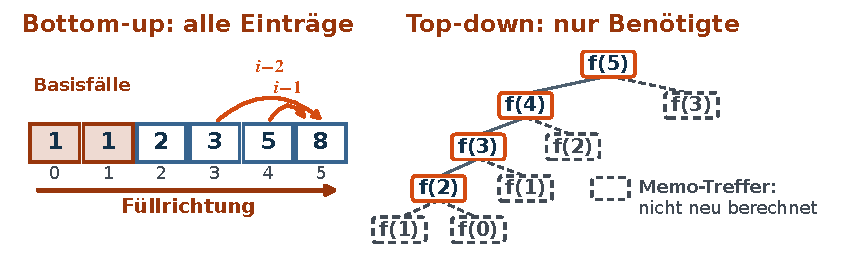
\includegraphics[width=\columnwidth]{Images/dynamic-programming-topdown-bottomup-fibonacci-fill.pdf}
\end{center}
\end{contentbox}

% ============================================================
% IMPLEMENTIERUNGSART UMBAUEN
% ============================================================

\subsection{Eine DP als Top-down oder Bottom-up}\label{sec:03-dp-umbauen}

\subsubsection{Zustand und Speicher festlegen}\label{sec:03-dp-zustand}

\begin{tablebox}[Funktionsparameter bestimmen den Zustand]
\begin{ZSFtable}[\ZSFfontTableDense]{Y{0.9} Y{0.9} Y{1.2}}
    \ZSFheaderRow
    \ZSFhead{Rekursion} & \ZSFhead{Memo-Schlüssel} & \ZSFhead{Bottom-up-Speicher} \\
    \texttt{solve(i)} & \texttt{i} & \texttt{dp[i]}: Liste \\
    \texttt{solve(i, j)} & \texttt{(i, j)} & \texttt{dp[i][j]}: Tabelle \\
    \texttt{solve(i, rest)} & \texttt{(i, rest)} & \texttt{dp[i][rest]}: Tabelle \\
    unregelmässige Zustände & unveränderliches Tupel & Dictionary mit demselben Schlüssel \\
\end{ZSFtable}
\end{tablebox}

\begin{contentbox}[Was gehört zum Zustand?]
Alle Parameter, die sich zwischen Aufrufen ändern und das Ergebnis beeinflussen. Unveränderte Eingaben wie \texttt{grid} oder \texttt{text} bleiben normale Argumente. \hl{Test:} Gleicher Memo-Schlüssel muss immer dasselbe Teilproblem und Ergebnis bedeuten; sonst fehlt ein Parameter im Zustand.
\end{contentbox}

\subsubsection{Basisfälle und ungültige Zustände}\label{sec:03-dp-basis}

\begin{tablebox}[Bekannte und unmögliche Zustände behandeln]
\begin{ZSFtable}[\ZSFfontTableDense]{Y{1.0} Y{1.0} Y{1.0}}
    \ZSFheaderRow
    \ZSFhead{Bedeutung} & \ZSFhead{Top-down} & \ZSFhead{Bottom-up} \\
    bekannter Basiswert & früher \texttt{return} & vor den Schleifen in \texttt{dp} eintragen \\
    ungültiger Zustand & passenden Wert zurückgeben & Zustand überspringen \\
    nicht erreichbar & \texttt{False}/Unendlich zurückgeben & gleicher Startwert in \texttt{dp} \\
\end{ZSFtable}
\end{tablebox}

\begin{contentbox}[Basiswert wählen]
Kleinstes direkt lösbares Teilproblem: leere Auswahl oft \texttt{0}, beim Zählen oft \texttt{1}, nicht erreichbar je nach Ziel \texttt{False}, \texttt{inf} oder \texttt{-inf}.
\end{contentbox}

\subsubsection{Vorgänger und Übergang bestimmen}\label{sec:03-dp-uebergang}

\begin{contentbox}[Was aus der Rekurrenz übernommen wird]
\begin{factlist}
\ZSFFact{Vorgänger}{Alle kleineren Zustände, deren Werte für den aktuellen Zustand gebraucht werden.}
\ZSFFact{Erlaubte Wahl}{Bedingungen aus der Aufgabe bleiben als \texttt{if} vor dem Aufruf beziehungsweise \texttt{dp}-Zugriff erhalten.}
\ZSFFact{Verknüpfung}{Möglichkeiten mit \texttt{max}, \texttt{min}, logischem Oder oder Addition verbinden.}
\end{factlist}
\end{contentbox}

\begin{codebox}[Derselbe Übergang in beiden Varianten]
\begin{lstlisting}[style=CodeExpert]
# Top-down: Vorgänger durch Aufruf holen
result = max(gain + solve(i-2, memo),
             solve(i-1, memo))

# Bottom-up: dieselben Vorgänger aus dp lesen
dp[i] = max(gain + dp[i-2],
            dp[i-1])
\end{lstlisting}
\end{codebox}

\subsubsection{Reine Rekursion als Ausgangslage}\label{sec:03-dp-reine-rekursion}
\begin{codebox}[Reine Rekursion zum Vergleich mit DP-Varianten]
\begin{lstlisting}[style=CodeExpert,escapeinside={(*@}{@*)}]
def solve(i, j):                  # Zustand (*@\ZSFref{sec:03-dp-zustand}@*)
    if ...:                          # Basis (*@\ZSFref{sec:03-dp-basis}@*)
        return ...
    # Vorgänger & Übergang (*@\ZSFref{sec:03-dp-uebergang}@*)
    # Richtung: Top-down via Rekursionspfad (*@\ZSFref{sec:03-dp-fuellrichtung}@*)
    # DP-Umbau: solve(prev) wird zu dp[prev] (Bottom-up)
    result = value + solve(prev_i, prev_j)
    return result                    # Ziel (*@\ZSFref{sec:03-dp-ziel}@*)
\end{lstlisting}
\end{codebox}

\ZSFmanualColumnBreak
\subsubsection{Rekursion mit Memoization ergänzen}\label{sec:03-dp-memoization}

Rekurrenz unverändert lassen: Zustand \ZSFref{sec:03-dp-zustand}, Basis \ZSFref{sec:03-dp-basis} und Übergang \ZSFref{sec:03-dp-uebergang} übernehmen; nur Lookup und Speichern ergänzen.

\begin{codebox}[Allgemeines Memoization-Gerüst]
\begin{lstlisting}[style=CodeExpert,escapeinside={(*@}{@*)}]
def solve(i, j, memo=None):
    if memo is None:                 # FEST: einmal erzeugen
        memo = {}
    state = (i, j)                   # Zustand (*@\ZSFref{sec:03-dp-zustand}@*)
    if state in memo:                # FEST: bereits berechnet?
        return memo[state]
    if ...:                          # Basis (*@\ZSFref{sec:03-dp-basis}@*)
        return ...
    # Vorgänger: Zustände, deren Werte wir brauchen
    # Übergang: rechte Seite der Rekurrenz übernehmen (*@\ZSFref{sec:03-dp-uebergang}@*)
    # Beispiel: Wert + Ergebnis des Vorgängers
    # bei JEDEM solve-Aufruf dasselbe memo mitgeben
    # if condition:  # ANPASSEN: falls nötig; result einrücken
    result = value + solve(prev_i, prev_j, memo)  # ANPASSEN
    memo[state] = result             # FEST: vor return speichern
    return result                    # Ziel (*@\ZSFref{sec:03-dp-ziel}@*)
\end{lstlisting}
\end{codebox}

\subsubsection{Dieselbe DP Bottom-up aufbauen}\label{sec:03-dp-bottom-up}

Zustand, Basis und Übergang bleiben gleich. Aufrufe werden zu \texttt{dp[prev]}; dazu Füllreihenfolge \ZSFref{sec:03-dp-fuellrichtung} wählen.

\begin{codebox}[Allgemeines Bottom-up-Gerüst]
\begin{lstlisting}[style=CodeExpert,escapeinside={(*@}{@*)}]
def solve_bottom_up(target):
    dp = {}                          # FEST: Wert pro Zustand
    dp[...] = ...                    # Basis (*@\ZSFref{sec:03-dp-basis}@*)
    # STATT Rekursion: Vorgänger vor aktuellem Zustand
    for i, j in states_in_order:     # Richtung (*@\ZSFref{sec:03-dp-fuellrichtung}@*)
        state = (i, j)               # Zustand (*@\ZSFref{sec:03-dp-zustand}@*)
        if state in dp:              # Basis nicht überschreiben
            continue
        # Vorgänger aus der Rekurrenz als dp-Schlüssel
        prev = (prev_i, prev_j)
        # dp[prev] liest seinen bereits berechneten Wert
        # if condition:  # ANPASSEN: falls nötig; result einrücken
        result = value + dp[prev]      # Übergang; ANPASSEN (*@\ZSFref{sec:03-dp-uebergang}@*)
        dp[state] = result            # FEST: Ergebnis speichern
    return dp[target]                # Ziel (*@\ZSFref{sec:03-dp-ziel}@*)
\end{lstlisting}
\end{codebox}

\subsubsection{Füllreihenfolge wählen}\label{sec:03-dp-fuellrichtung}

\begin{tablebox}[Füllrichtung aus den Vorgängern ablesen]
\begin{ZSFtable}[\ZSFfontTableDense]{Y{0.9} Y{1.1}}
    \ZSFheaderRow
    \ZSFhead{Zustand braucht} & \ZSFhead{Achse füllen} \\
    kleinere Indizes wie \texttt{i-1}, \texttt{i-k} & \texttt{i} aufsteigend \\
    grössere Indizes wie \texttt{i+1}, \texttt{i+k} & \texttt{i} absteigend \\
    \texttt{(i-a, j-b)} & betroffene Achsen aufsteigend \\
    \texttt{(i+a, j-b)} & \texttt{i} absteigend, \texttt{j} aufsteigend \\
\end{ZSFtable}
\end{tablebox}

\begin{contentbox}[Top-down]
Keine Schleifenrichtung: Der Zielaufruf folgt den Vorgängern rekursiv bis zur Basis. Bottom-up muss jeden gelesenen \texttt{dp}-Wert vorher berechnen.
\end{contentbox}

\subsubsection{Zielwert lesen und Varianten übersetzen}\label{sec:03-dp-ziel}

\begin{tablebox}[Dieselben Bausteine in beiden Varianten]
\begin{ZSFtable}[\ZSFfontTableDense]{Y{1.1} Y{0.95} Y{0.95}}
    \ZSFheaderRow
    \ZSFhead{Baustein} & \ZSFhead{Memoization} & \ZSFhead{Bottom-up} \\
    Zustand \ZSFref{sec:03-dp-zustand} & Schlüssel \texttt{state} & Index/Schlüssel von \texttt{dp} \\
    Basisfall \ZSFref{sec:03-dp-basis} & früher \texttt{return} & vorab in \texttt{dp} eintragen \\
    Vorgänger \ZSFref{sec:03-dp-uebergang} & \texttt{solve(prev, memo)} & \texttt{dp[prev]} \\
    Reihenfolge \ZSFref{sec:03-dp-fuellrichtung} & rekursive Aufrufe & passende Schleifen \\
    Ziel \ZSFref{sec:03-dp-ziel} & \texttt{solve(target)} & \texttt{dp[target]} \\
\end{ZSFtable}
\end{tablebox}

\begin{contentbox}[Was bleibt, was ändert sich?]
\begin{factlist}
\ZSFFact{Bleibt gleich}{Bedeutung des Zustands, Basiswerte, Vorgänger, erlaubte Wahl, Verknüpfung und gesuchtes Ziel.}
\ZSFFact{Ändert sich}{Memo-Lookup und rekursive Aufrufe werden zu vorgefüllten Basiswerten, \texttt{dp}-Zugriffen und Schleifen.}
\ZSFFact{Zurück zu Top-down}{\texttt{dp}-Indizes werden Parameter, Basiszellen frühe Rückgaben und \texttt{dp[prev]} rekursive Aufrufe; Schleifen entfallen \ZSFref{sec:03-dp-memoization}.}
\end{factlist}
\end{contentbox}

% ============================================================
% LÖSUNGSREZEPT UND GENERISCHE SKELETTE
% ============================================================

\ZSFmanualColumnBreak
\subsection{Start hier: Aufgabe erkennen}\label{sec:03-loesungsrezept}
\ZSFindex{Rekonstruktion}

\begin{factlist}
\ZSFFact{\texttt{FEST}}{Grundstruktur der DP-Familie; normalerweise übernehmen.}
\ZSFFact{\texttt{ANPASSEN}}{Diese Zeile hängt von Zustand, Basis, Übergang oder Ziel der Aufgabe ab.}
\ZSFFact{\texttt{OPTIONnn}}{Nummeriertes Zusatzfeature eines Skeletons. Nur für den erklärten Fall alle Zeilen mit derselben Nummer einkommentieren.}
\end{factlist}

\begin{tablebox}[Was steht in der Aufgabe? → Direkt zum Beispiel]
\begin{ZSFtable}[\ZSFfontTableDense]{Y{1.45} Y{0.7} Y{0.85}}
    \ZSFheaderRow
    \ZSFhead{Typische Formulierung} & \ZSFhead{Gesucht} & \ZSFhead{Direkt zu} \\
    Rekursiver Code gegeben; Memoization oder Bottom-up verlangt & gleiche Lösung & \ZSFsectionref{sec:03-dp-umbauen}\ Umbauen \\
    Mathematische \ZSFkeyword*{Rekurrenz} gegeben; implementieren & Funktionswert & \ZSFsectionref{sec:03-fibonacci}\ Rekurrenz \\
    Pro Position \ZSFkeyword*{wählen oder auslassen}; \ZSFkeyword*{Nachbarn verboten} & grösster Wert & \ZSFsectionref{sec:03-house-robber}\ House Robber \\
    Gegenstände \ZSFkeyword*{höchstens einmal} wählen; \ZSFkeyword*{Kapazitätslimit} & grösster Wert & \ZSFsectionref{sec:03-knapsack}\ Knapsack \\
    Zahlen \ZSFkeyword*{höchstens einmal} verwenden; Zielsumme erreichen & Ja / Nein & \ZSFsectionref{sec:03-subset-sum}\ Subset Sum \\
    Betrag mit denselben Münzen \ZSFkeyword*{beliebig oft} aufbauen & kleinste Anzahl & \ZSFsectionref{sec:03-coin-change}\ Coin Change \\
    Anzahl verschiedener Münzkombinationen bestimmen & Anzahl & \ZSFsectionref{sec:03-coin-combinations}\ Kombinationen \\
    Anzahl verschiedener Reihenfolgen bestimmen & Anzahl & \ZSFsectionref{sec:03-coin-combinations}\ Reihenfolgen \\
    Länge in Stücke mit gegebenen Werten zerlegen & grösster Wert & \ZSFsectionref{sec:03-rod-cutting}\ Rod Cutting \\
    Werte \ZSFkeyword*{beliebig oft} verwenden; erreichbare Beträge & Ja / Nein & \ZSFsectionref{sec:03-reachable-amounts}\ Reachable \\
    \ZSFkeyword*{Zwei Strings oder Listen} vergleichen & Länge & \ZSFsectionref{sec:03-lcs}\ LCS-Länge \\
    Konkrete gemeinsame Teilfolge ausgeben & Länge + Folge & \ZSFsectionref{sec:03-lcs}\ LCS-Folge \\
    \ZSFkeyword*{Durch ein Gitter bewegen}; Werte maximieren, Zellen gesperrt & grösster Wert & \ZSFsectionref{sec:03-grid-min-path}\ Grid-Wert \\
\end{ZSFtable}
\end{tablebox}

\begin{tablebox}[Gesuchtes Resultat → Verknüpfung]
\begin{ZSFtable}[\ZSFfontTableDense]{Y{0.8} Y{0.7} Y{1.5}}
    \ZSFheaderRow
    \ZSFhead{Frage} & \ZSFhead{Operation} & \ZSFhead{Startwert} \\
    bester Wert & \texttt{max} & \texttt{-float("inf")} \\
    kleinste Kosten & \texttt{min} & \texttt{float("inf")} \\
    erreichbar? & logisches Oder & \texttt{False}; Start \texttt{True} \\
    Anzahl Möglichkeiten & Addition & \texttt{0}; Start \texttt{1} \\
\end{ZSFtable}
\end{tablebox}

% ============================================================
% 1D-DP
% ============================================================

\subsection{1D-DP: \texttt{dp[i]} — Lineare Sequenzen}\label{sec:03-1d-dp}

\begin{contentbox}[Musterkarte]
\begin{factlist}
\ZSFFact{Ziel}{Für jede Position das beste Ergebnis bis dorthin speichern, damit die Lösung am Ende der Reihe feststeht.}
\ZSFFact{Zustand}{\texttt{dp[i]} = Lösung bis Position beziehungsweise Grösse \texttt{i}.}
\ZSFFact{Feste Vorgänger}{Nur frühere Werte wie \texttt{i-1}, \texttt{i-2}: \ZSFsectionref{sec:03-fibonacci} Fibonacci.}
\ZSFFact{Nehmen/Auslassen}{Aktuelles Element wählen oder überspringen: \ZSFsectionref{sec:03-house-robber} House Robber.}
\ZSFFact{Aufwand}{Meist $O(n)$ Zeit und $O(n)$ Speicher.}
\end{factlist}
\end{contentbox}

\subsubsection{Rekurrenzen / feste Vorgänger}\label{sec:03-fibonacci}
\ZSFindex{Fibonacci}
\ZSFindex{Rekurrenz}

\begin{contentbox}[Muster: mathematische Rekurrenz übertragen]
\begin{factlist}
\ZSFFact{Erkennen}{Eine Folge oder Funktion ist durch Basisfälle und eine Formel mit früheren Werten wie \texttt{P(n-1)} oder \texttt{P(n-2)} definiert.}
\ZSFFact{Basisfälle}{Bekannte Werte direkt in \texttt{memo} beziehungsweise \texttt{dp} eintragen.}
\ZSFFact{Übertragen}{Jedes \texttt{P(n-k)} wird zum rekursiven Aufruf; Faktoren, Rechenzeichen und Vergleiche unverändert übernehmen.}
\ZSFFact{Top-down}{Wenn Rekursion oder Memoization verlangt ist: vom Ziel aus rechnen und jeden neuen Wert speichern.}
\ZSFFact{Bottom-up}{Wenn Iteration erlaubt ist: ab den Basisfällen vorwärts rechnen.}
\end{factlist}
\end{contentbox}

\begin{codebox}[Top-down: Memoization]
\begin{lstlisting}[style=CodeExpert]
def recurrence_memo(n, memo=None):
    # ANPASSEN: alle Basisfälle aus der Aufgabe
    if memo is None:
        memo = {0: ..., 1: ...}

    # FEST: bekannten Wert nicht erneut berechnen
    if n in memo:
        return memo[n]

    # ANPASSEN: rechte Seite der Rekurrenz direkt einsetzen
    # P(n-k) wird zu recurrence_memo(n-k, memo)
    memo[n] = ...
    return memo[n]
\end{lstlisting}
\end{codebox}

\begin{contentbox}[Memoization: typische Fehler]
\begin{factlist}
\ZSFFact{Gleicher Speicher}{In jedem rekursiven Aufruf dasselbe \texttt{memo} weitergeben.}
\ZSFFact{Standardargument}{\texttt{memo=None} verwenden und das Dictionary erst in der Funktion erzeugen.}
\ZSFFact{Formel}{Faktoren, Minuszeichen und Klammern aus der Rekurrenz nicht verlieren.}
\ZSFFact{Reihenfolge}{Wert berechnen, in \texttt{memo[n]} speichern und danach zurückgeben.}
\end{factlist}
\end{contentbox}

\begin{codebox}[Bottom-up: Rekurrenz vorwärts berechnen]
\begin{lstlisting}[style=CodeExpert]
def recurrence_bottom_up(n):
    # ANPASSEN: alle Basisfälle aus der Aufgabe
    dp = [None] * (n + 1)
    dp[0] = ...
    if n >= 1:
        dp[1] = ...

    # FEST: nach den Basisfällen vorwärts rechnen
    for i in range(2, n + 1):
        # ANPASSEN: P(i-k) wird zu dp[i-k]
        dp[i] = ...
    return dp[n]
\end{lstlisting}
\end{codebox}

\subsubsection{House Robber / Coin Row}\label{sec:03-house-robber}

\begin{contentbox}[Muster: nehmen oder weglassen]
\begin{factlist}
\ZSFFact{Problem}{Keine zwei direkt benachbarten Werte gleichzeitig wählen; Summe maximieren.}
\ZSFFact{Weglassen}{Bestes Ergebnis bis zum Vorgänger: \texttt{dp[i-1]}.}
\ZSFFact{Nehmen}{Aktueller Wert plus bestes Ergebnis vor dem verbotenen Abstand.}
\ZSFFact{Anpassen}{\texttt{min\_distance=2} verbietet direkte Nachbarn; für grössere Sperrabstände erhöhen. Basis und \texttt{max}/\texttt{min} an die Aufgabe anpassen.}
\end{factlist}
\end{contentbox}

\begin{codebox}[Maximaler Wert: Nehmen/Auslassen]
\begin{lstlisting}[style=CodeExpert]
def house_robber(nums, min_distance=2):
    # nums[i] = Wert an Position i
    num_positions = len(nums)
    if num_positions == 0:
        return 0
    # FEST: Zustand und Basis für die ersten i Elemente
    dp = [0] * (num_positions + 1)
    dp[0], dp[1] = 0, nums[0]
    # FEST: pro Position weglassen oder nehmen
    for i in range(2, num_positions + 1):
        skip = dp[i-1]               # ANPASSEN: weglassen
        previous = max(0, i-min_distance)  # ANPASSEN: Abstand
        take = dp[previous] + nums[i-1]    # ANPASSEN: nehmen
        dp[i] = max(skip, take)       # ANPASSEN: Ziel
    return dp[num_positions]
\end{lstlisting}
\end{codebox}

% ============================================================
% KAPAZITÄTS- UND BETRAGS-DP
% ============================================================

\subsection{Kapazitäts- und Betrags-DP}\label{sec:03-kapazitaets-dp}

\begin{contentbox}[Musterkarte]
\begin{factlist}
\ZSFFact{Ziel}{Mit den verfügbaren Objekten oder Beträgen den besten Wert finden oder einen gewünschten Betrag erreichen.}
\ZSFFact{0/1-Auswahl}{Jedes Objekt höchstens einmal: \ZSFsectionref{sec:03-knapsack} Knapsack.}
\ZSFFact{0/1-Erreichbarkeit}{Jede Zahl höchstens einmal: \ZSFsectionref{sec:03-subset-sum} Subset Sum.}
\ZSFFact{Wiederholbare Wahl}{Dieselbe Wahl beliebig oft: \ZSFsectionref{sec:03-coin-change} Coin Change.}
\ZSFFact{Wiederholbarer Wert}{Besten Wert mit beliebig oft nutzbaren Teilen: \ZSFsectionref{sec:03-rod-cutting} Rod Cutting.}
\ZSFFact{Wiederholbare Erreichbarkeit}{Erreichbare Beträge mit beliebig vielen Wiederholungen: \ZSFsectionref{sec:03-reachable-amounts} Reachable Amounts.}
\end{factlist}
\end{contentbox}

\begin{tablebox}[Eine Betragsachse: Was ändert sich?]
\begin{ZSFtable}[\ZSFfontTableDense]{Y{1.0} Y{0.8} Y{1.2}}
    \ZSFheaderRow
    \ZSFhead{Aufgabe} & \ZSFhead{Nutzung} & \ZSFhead{Kernänderung} \\
    0/1-Maximum & höchstens einmal & vorherige Tabellenzeile \\
    0/1-erreichbar & höchstens einmal & Beträge rückwärts, Oder \\
    Minimum & beliebig oft & kleinere Beträge vorwärts, \texttt{min} \\
    erreichbar & beliebig oft & kleinere Beträge vorwärts, Oder \\
    Anzahl Kombinationen & beliebig oft & Münzen aussen, Addition \\
    Maximum & beliebig oft & kleinere Beträge vorwärts, \texttt{max} \\
\end{ZSFtable}
\end{tablebox}

\subsubsection{0/1 Knapsack}\label{sec:03-knapsack}

\begin{contentbox}[Muster: nehmen oder weglassen]
\begin{factlist}
\ZSFFact{Entscheidung}{Weglassen \texttt{dp[i-1][w]} oder Nehmen \texttt{values[i-1] + dp[i-1][w-weights[i-1]]}.}
\ZSFFact{Anpassen}{Gewichte, Werte, Basis, \texttt{max}/\texttt{min}; vorige Zeile macht Auswahl zu 0/1.}
\end{factlist}
\end{contentbox}

\begin{codebox}[Maximaler Wert: 0/1-Auswahl]
\begin{lstlisting}[style=CodeExpert]
def knapsack(weights, values, capacity):
    # weights[i] und values[i] gehören zum selben Objekt
    num_items = len(values)
    # FEST: Zustand und Basis für 0 Objekte
    dp = [[0] * (capacity + 1)
          for _ in range(num_items + 1)]
    # FEST: jede Zelle aus Auslassen oder Nehmen bilden
    for i in range(1, num_items + 1):  # FEST: Objektachse
        for w in range(capacity + 1):  # FEST: Betragsachse
            dp[i][w] = dp[i-1][w]      # ANPASSEN: AUSLASSEN
            if weights[i-1] <= w:      # ANPASSEN: erlaubt?
                dp[i][w] = max(
                    dp[i][w],
                    values[i-1] + dp[i-1][w-weights[i-1]]
                )                       # ANPASSEN: NEHMEN + Ziel
    return dp[num_items][capacity]        # maximaler Wert
\end{lstlisting}
\end{codebox}

\subsubsection{Subset Sum: 0/1-Erreichbarkeit}\label{sec:03-subset-sum}

\begin{codebox}[Ja/Nein: jede Zahl höchstens einmal]
\begin{lstlisting}[style=CodeExpert]
def subset_sum(numbers, target):
    # FEST: Boolean-Zustand; nur Summe 0 ist anfangs erreichbar
    reachable = [False] * (target + 1)
    reachable[0] = True
    for number in numbers:              # FEST: jede Zahl ansehen
        # ANPASSEN: genau eine der beiden Richtungen wählen
        amounts = range(target, number-1, -1) # 0/1: rückwärts
        # amounts = range(number, target+1)   # wiederholbar
        for amount in amounts:
            # ANPASSEN: weglassen ODER nehmen
            reachable[amount] = (reachable[amount]
                                 or reachable[amount-number])
    return reachable[target]            # Ziel erreichbar?
\end{lstlisting}
\end{codebox}

\subsubsection{Coin Change: wiederholbare Wahl}\label{sec:03-coin-change}

\begin{codebox}[Minimale Anzahl: wiederholbare Wahl]
\begin{lstlisting}[style=CodeExpert]
def coin_change(coin_values, target_amount):
    # coin_values = erlaubte Werte; target_amount = Ziel
    # FEST: Minimum-Zustand; Betrag 0 kostet keine Münze
    dp = [float("inf")] * (target_amount + 1)
    dp[0] = 0
    # FEST: Beträge vorwärts aus kleineren Beträgen bauen
    for amount in range(1, target_amount + 1):
        for coin in coin_values:        # ANPASSEN: erlaubte Wahl
            if coin <= amount:          # ANPASSEN: erlaubt?
                candidate = dp[amount-coin] + 1
                dp[amount] = min(dp[amount], candidate)  # Ziel
    if dp[target_amount] == float("inf"):
        return -1
    return dp[target_amount]      # kleinste Münzanzahl
\end{lstlisting}
\end{codebox}

\subsubsection{Coin Change: Kombinationen oder Reihenfolgen}\label{sec:03-coin-combinations}

\begin{contentbox}[Entscheidender Unterschied]
\begin{factlist}
\ZSFFact{Kombinationen}{Münzen aussen: \texttt{1+2} und \texttt{2+1} zählen zusammen nur einmal.}
\ZSFFact{Reihenfolgen}{Beträge aussen: \texttt{1+2} und \texttt{2+1} zählen als zwei Möglichkeiten.}
\ZSFFact{Anpassen}{Erlaubte Werte, Zielbetrag, Basis \texttt{ways[0]=1} und Addition.}
\end{factlist}
\end{contentbox}

\begin{codebox}[Anzahl: Kombinationen oder Reihenfolgen]
\begin{lstlisting}[style=CodeExpert]
def count_coin_combinations(coin_values, target_amount):
    # FEST: Zählzustand; die leere Auswahl zählt für Betrag 0
    ways = [0] * (target_amount + 1)
    ways[0] = 1
    # FEST für Kombinationen: jede Münze als Typ öffnen
    for coin in coin_values:
        # FEST für Wiederholung: Beträge vorwärts
        for amount in range(coin, target_amount + 1):
            ways[amount] += ways[amount-coin]  # ANPASSEN: zählen
    return ways[target_amount]

def count_coin_sequences(coin_values, target_amount):
    # FEST: gleicher Zählzustand, aber andere Schleifenreihenfolge
    ways = [0] * (target_amount + 1)
    ways[0] = 1
    # FEST für Reihenfolgen: jeden Betrag der Reihe nach öffnen
    for amount in range(1, target_amount + 1):
        for coin in coin_values:
            if coin <= amount:
                ways[amount] += ways[amount-coin] # ANPASSEN
    return ways[target_amount]
\end{lstlisting}
\end{codebox}

\subsubsection{Rod Cutting: maximaler Wert}\label{sec:03-rod-cutting}

\begin{contentbox}[Muster: Teile beliebig oft verwenden]
\begin{factlist}
\ZSFFact{Zustand}{\texttt{dp[length]} = bester Wert für genau diese Gesamtlänge.}
\ZSFFact{Übergang}{Passendes Stück anhängen: Stückwert plus bester Wert der Restlänge.}
\ZSFFact{Anpassen}{Erlaubte Stücklängen, zugehörige Werte, Ziellänge und \texttt{max}/\texttt{min}.}
\end{factlist}
\end{contentbox}

\begin{codebox}[Bester Wert: wiederholbare Stücke]
\begin{lstlisting}[style=CodeExpert]
def rod_cut(piece_lengths, piece_values, target_length):
    # FEST: Länge 0 hat Wert 0; andere noch unerreichbar
    dp = [-float("inf")] * (target_length + 1)
    dp[0] = 0

    # FEST: kleinere Längen vor grösseren berechnen
    for length in range(1, target_length + 1):
        for piece, value in zip(piece_lengths, piece_values):
            if piece <= length:             # Stück passt?
                candidate = value + dp[length-piece]
                dp[length] = max(dp[length], candidate)

    return dp[target_length]                 # maximaler Wert
\end{lstlisting}
\end{codebox}


\subsubsection{Reachable Amounts: Boolean-DP}\label{sec:03-reachable-amounts}

\begin{codebox}[Ja/Nein: Werte beliebig oft]
\begin{lstlisting}[style=CodeExpert]
def reachable_amounts(coin_values, limit):
    # coin_values dürfen wiederholt werden; prüfe 0..limit
    # FEST: Boolean-Zustand; nur Betrag 0 ist anfangs erreichbar
    reachable = [False] * (limit + 1)
    reachable[0] = True
    # FEST: Beträge vorwärts aus kleineren Beträgen bauen
    for amount in range(1, limit + 1):
        for coin in coin_values:        # ANPASSEN: erlaubte Wahl
            if amount >= coin and reachable[amount-coin]:
                reachable[amount] = True  # ANPASSEN: erreichbar
                break
    return reachable              # Boolean-Antwort für jeden Betrag
\end{lstlisting}
\end{codebox}

% ============================================================
% ZWEI PRÄFIXE
% ============================================================

\subsection{Zwei Präfixe: \texttt{dp[i][j]}}\label{sec:03-zwei-praefixe}
\ZSFindex{Zwei-Index-DP}

\begin{contentbox}[Musterkarte]
\begin{factlist}
\ZSFFact{Ziel}{Zwei Folgen schrittweise vergleichen und die beste gemeinsame Lösung für ihre Präfixe aufbauen.}
\ZSFFact{Zustand}{\texttt{dp[i][j]} = Lösung für Präfix \texttt{i} von \texttt{A} und Präfix \texttt{j} von \texttt{B}.}
\ZSFFact{Gleich}{Diagonal weitergehen; bei LCS kommt ein Treffer hinzu.}
\ZSFFact{Ungleich}{Eine Seite auslassen und den besseren Vorgänger wählen.}
\ZSFFact{Anpassen}{Basiszeile/-spalte sowie Übergänge bei Gleichheit und Ungleichheit bestimmen die konkrete Zwei-Präfix-Aufgabe.}
\ZSFFact{OPTION01: Folge ausgeben}{Nur wenn die konkrete gemeinsame Folge verlangt ist: alle \texttt{OPTION01}-Zeilen einkommentieren und die Rekonstruktion verwenden.}
\ZSFFact{Skeleton}{\ZSFsectionref{sec:03-lcs} LCS für zwei Strings oder Listen.}
\end{factlist}
\end{contentbox}

\subsubsection{Longest Common Subsequence (LCS): Länge}\label{sec:03-lcs}
\ZSFindex[lcs]{LCS / Longest Common Subsequence}
\ZSFindex{Rekonstruktion}

\begin{codebox}[Länge der LCS: Bottom-up-Skeleton]
\begin{lstlisting}[style=CodeExpert]
def lcs(sequence_a, sequence_b):
    # Eingaben sind zwei Strings oder Listen
    len_a, len_b = len(sequence_a), len(sequence_b)
    # FEST: Präfixzustand; ein leeres Präfix hat Wert 0
    dp = [[0] * (len_b + 1) for _ in range(len_a + 1)]
    # FEST: alle Präfixpaare zeilenweise füllen
    for i in range(1, len_a + 1):       # FEST: Präfix A
        for j in range(1, len_b + 1):   # FEST: Präfix B
            # ANPASSEN: gleich -> diagonal; ungleich -> oben/links
            if sequence_a[i-1] == sequence_b[j-1]:
                dp[i][j] = dp[i-1][j-1] + 1
            else:
                dp[i][j] = max(dp[i-1][j],
                               dp[i][j-1])
    # return dp[len_a][len_b], dp  # OPTION01
    return dp[len_a][len_b]        # Standard: nur Länge
\end{lstlisting}
\end{codebox}

\begin{codebox}[OPTION01: konkrete LCS rekonstruieren]
\begin{lstlisting}[style=CodeExpert]
def reconstruct_lcs(sequence_a, sequence_b, dp):
    i, j = len(sequence_a), len(sequence_b)
    chosen = []
    # FEST: vom Ziel rückwärts bis ein Präfix leer ist
    while i > 0 and j > 0:
        if sequence_a[i-1] == sequence_b[j-1]:
            chosen.append(sequence_a[i-1])  # MATCH gewählt
            i, j = i - 1, j - 1
        elif dp[i-1][j] >= dp[i][j-1]:
            i -= 1                       # A-Wert auslassen
        else:
            j -= 1                       # B-Wert auslassen
    chosen.reverse()
    return chosen
\end{lstlisting}
\end{codebox}

% ============================================================
% GRID-DP
% ============================================================

\subsection{Grid-DP: \texttt{dp[i][j]}}\label{sec:03-grid-dp}
\ZSFindex{Grid-DP}

\begin{contentbox}[Musterkarte]
\begin{factlist}
\ZSFFact{Ziel}{Einen optimalen Weg durchs Gitter finden, der erlaubte Zellen nutzt und gesperrte Zellen meidet.}
\ZSFFact{Zustand}{\texttt{dp[row][col]} = bester Wert vom Start bis zu dieser Zelle.}
\ZSFFact{Schnell oder flexibel}{Wenige feste Vorgänger direkt einsetzen; bei variablen oder vielen Bewegungen den \texttt{FLEX}-Block mit \texttt{moves} verwenden.}
\ZSFFact{Füllrichtung}{Spalten von links nach rechts, darin Zeilen von oben nach unten; jede Bewegung muss auf bereits berechnete Zellen zeigen.}
\ZSFFact{Anpassen}{\texttt{moves}, \texttt{blocked}, \texttt{start}, Füllrichtung, Zellbeitrag, \texttt{max}/\texttt{min} und Zielauslese.}
\ZSFFact{Grenze}{Erzeugen Bewegungen Zyklen, braucht es einen zusätzlichen Zustand oder einen Graphalgorithmus.}
\end{factlist}
\end{contentbox}

\subsubsection{Grid-Wert: maximale Belohnung mit Sperren}\label{sec:03-grid-min-path}

\begin{codeboxfirst}[Bottom-up-Skeleton: Initialisierung]
\begin{lstlisting}[style=CodeExpert]
# ANPASSEN: Bewegung = (Zeilenänderung, Spaltenänderung)
moves = [(1, 0), (0, 1)]          # unten, rechts

def grid_dp(grid, moves, blocked=-1, start=(0, 0)):
    rows, cols = len(grid), len(grid[0])
    start_row, start_col = start        # ANPASSEN: Start
    # FEST: bester Wert vom Start bis zu jeder Zelle
    # None bedeutet: Zelle bisher nicht erreichbar
    dp = [[None] * cols for _ in range(rows)]
    # ANPASSEN: erreichbaren Start als Basis setzen
    if grid[start_row][start_col] != blocked:
        dp[start_row][start_col] = grid[start_row][start_col]
\end{lstlisting}
\end{codeboxfirst}

\begin{codeboxlast}[Bottom-up-Skeleton: Vorgänger \& Füllen]
\begin{lstlisting}[style=CodeExpert]
    # ANPASSEN: Füllrichtung muss zu moves passen
    for col in range(cols):                    # links -> rechts
        for row in range(rows):                # oben -> unten
            if (row, col) == start or grid[row][col] == blocked:
                continue
            prev = []                       # erreichbare Vorgänger
            # FLEX: moves rückwärts -> mögliche Vorgänger
            for row_change, col_change in moves:
                prev_row = row - row_change
                prev_col = col - col_change
                inside = (0 <= prev_row < rows
                          and 0 <= prev_col < cols)
                if inside and dp[prev_row][prev_col] is not None:
                    prev.append((prev_row, prev_col))
            if not prev:                      # bleibt unerreichbar
                continue
            # ANPASSEN: max für Belohnung, min für Kosten
            # key vergleicht die dp-Werte der Vorgänger
            best = max(
                prev,
                key=lambda pos: dp[pos[0]][pos[1]])
            prev_row, prev_col = best
            dp[row][col] = (dp[prev_row][prev_col]
                            + grid[row][col])  # ANPASSEN: Übergang
    return dp                                   # Standard: nur Werte
\end{lstlisting}
\end{codeboxlast}

\begin{codebox}[SCHNELL: ersetzt nur den FLEX-Block]
\begin{lstlisting}[style=CodeExpert]
# Beispiel unten/rechts: feste Vorgänger oben/links
if row > 0 and dp[row-1][col] is not None:
    prev.append((row-1, col))  # von oben
if col > 0 and dp[row][col-1] is not None:
    prev.append((row, col-1))  # von links
\end{lstlisting}
\end{codebox}

\begin{codebox}[Ziel auslesen]
\begin{lstlisting}[style=CodeExpert]
# Eine Zielzelle
return dp[target_row][target_col]

# Mehrere mögliche Ziele
values = [dp[row][col] for row, col in targets
          if dp[row][col] is not None]
return max(values)                 # ANPASSEN: max oder min
\end{lstlisting}
\end{codebox}

%%%%%%%%%%%%%%%%%%%%%%%%%%%%%%%%%%%%%%%%%%%%%%%%%%%%%%%%%%%%%%%%%%%%%%%%%%%%%%%%%%%%%%%%%%%%%%%%%%%%%%%%%%%%%%%%%%%%%%
% Farb-Theme für Sections ab Kapitel 04 (Blaugrün)
